\section*{Pregunta 2}
\noindent Muestra que dado un conjunto $T$ de $n$ nodos $x_1, x_2, \dots, x_n$ con valores y prioridades distintas, el árbol treap asociado a $T$ es único. Hint: utiliza inducción sobre $n$.

\subsection*{Respuesta}

\textbf{Demostración por contradicción:}
Suponer que para $T$ tenemos más de un árbol treap asociado. Entonces $G$ y $G'$ son árboles asociados a $T$, entonces $V(G)=V(G')=T=\{x_1, x_2, \dots, x_n\}$, luego tenemos que $E(G)=E(G')$ dado que si $x_2 \prec x_1$,es decir que $x_2$ sea hijo de $x_1$, entonces $y_2 \prec y_1$, es decir $y_2$ es hijo de $y_1$. En el siguiente árbol podemos observar lo anterior ademas de que $x_2 < x_1$ y por tanto $y_2 < y_1$:

\begin{figure}[h!]
    \centering
    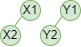
\includegraphics[width=0.2\textwidth]{t1-3.jpg}
\end{figure}
Por lo que $e(x_1,x_2)=e(y_1,y_2)$ para todos los vértices en $G=G'$. Entonces $G=G'$ lo cual es una contradicción al suponer que el árbol treap asociado a $T$ no es único, por tanto si es único. 
\bigskip
